\documentclass[runningheads]{llncs}
\usepackage{graphicx}
\usepackage{booktabs}
\usepackage{multirow}
\usepackage{xcolor}
\usepackage{colortbl}
\usepackage{amsmath}

\begin{document}

\title{Supplementary Material:\\Topology-Aware Fine-Tuning of CT Foundation Models\\for Coronary Artery Segmentation}
\titlerunning{Supplementary Material}
\maketitle

%----------------------------------------------------------------------
% ImageCAS block (§1–§4)
%----------------------------------------------------------------------

\section{$\lambda{=}0$ Continued-Training Controls}
\label{sec:lambda0}

To isolate the effect of the topology loss from the effect of continued training at LR$\,{=}\,10^{-5}$ from the L1 checkpoint, we train two control models with $\lambda_s{=}0$ (all other hyperparameters matched):

\begin{itemize}
\item \textbf{Frozen $\lambda{=}0$}: Decoder-only training, 30 epochs, LR$\,{=}\,10^{-5}$, no topology loss.
\item \textbf{Full $\lambda{=}0$}: Full fine-tuning, 30 epochs, LR$\,{=}\,10^{-5}$, no topology loss.
\end{itemize}

Table~\ref{tab:lambda0} compares these controls against the corresponding topology-trained models.

\begin{table}[h]
\caption{$\lambda{=}0$ continued-training controls vs.\ topology-trained models on ImageCAS ($n{=}250$ test). If continued training alone improves BCS, the $\lambda{=}0$ control should match the topology-trained model.}
\label{tab:lambda0}
\centering
\small
\begin{tabular}{llccccc}
\toprule
Adaptation & $\lambda_s$ & Dice $\uparrow$ & BCS $\uparrow$ & HD95\,(mm) $\downarrow$ & Betti$_0$ $\downarrow$ \\
\midrule
\multicolumn{2}{l}{\textit{L1 baseline}} & 0.792 & 0.688 & 6.7 & 5.02 \\
\midrule
Frozen & 0 (control)  & \textit{TBD} & \textit{TBD} & \textit{TBD} & \textit{TBD} \\
Frozen & 0.05 (BCS)   & 0.792 & 0.722 & 8.8 & 9.11 \\
\midrule
Full   & 0 (control)  & \textit{TBD} & \textit{TBD} & \textit{TBD} & \textit{TBD} \\
Full   & 0.10 (BCS)   & 0.797 & 0.735 & 6.7 & 5.66 \\
\bottomrule
\end{tabular}
\end{table}

\textit{Results pending (Job 8409). Expected: $\lambda{=}0$ controls will show minimal BCS improvement over L1, confirming that the topology loss---not continued training---drives the BCS gains observed in the main paper.}

%----------------------------------------------------------------------
\section{Training Curves}
\label{sec:training_curves}

Figure~\ref{fig:training_curves} shows validation Dice and total loss across training epochs for representative configurations.

\begin{figure}[h]
\centering
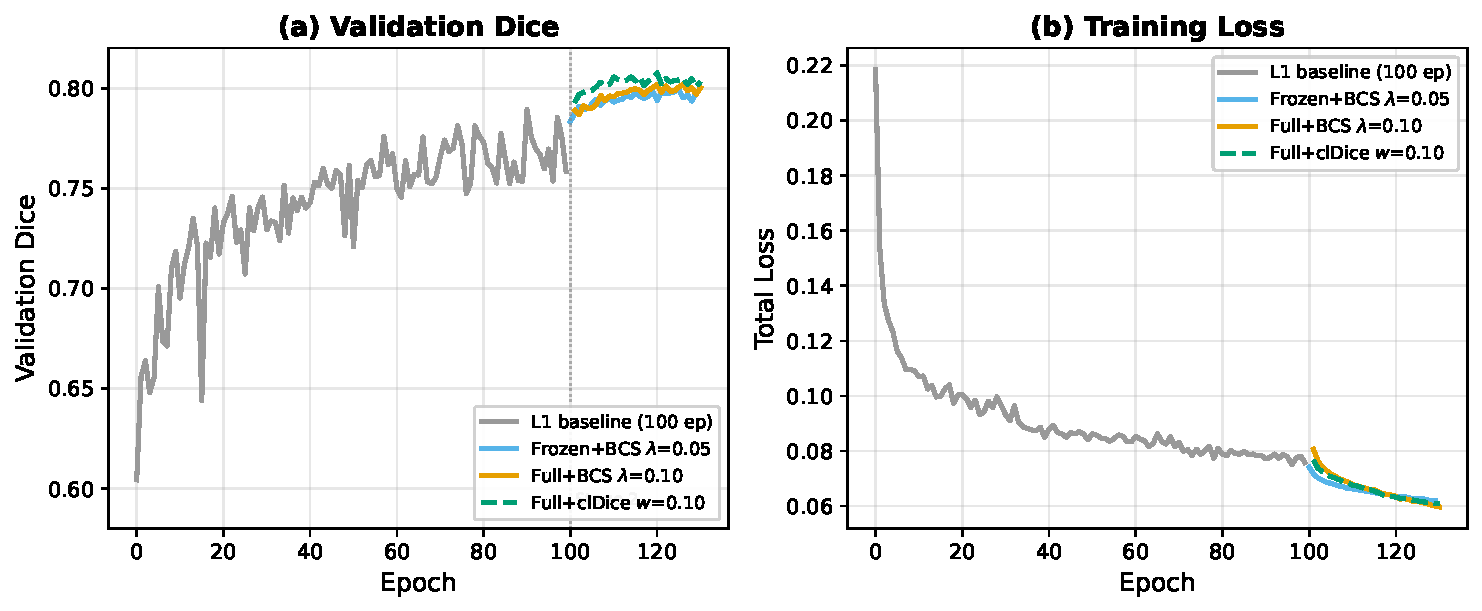
\includegraphics[width=\linewidth]{../figures/supp_training_curves.pdf}
\caption{Two-stage training curriculum. \textbf{(a)}~L1 baseline trains for 100 epochs; stage-2 models initialise from L1 and continue for 30 epochs (101--130). All stage-2 variants converge within 10--15 epochs. \textbf{(b)}~Total loss shows the stage-2 models start from L1's converged loss and further decrease with topology supervision.}
\label{fig:training_curves}
\end{figure}

%----------------------------------------------------------------------
\section{Per-Case Distribution}
\label{sec:per_case}

Figure~\ref{fig:per_case} shows per-case Dice and BCS distributions across the 250 test cases for key configurations.

\begin{figure}[h]
\centering
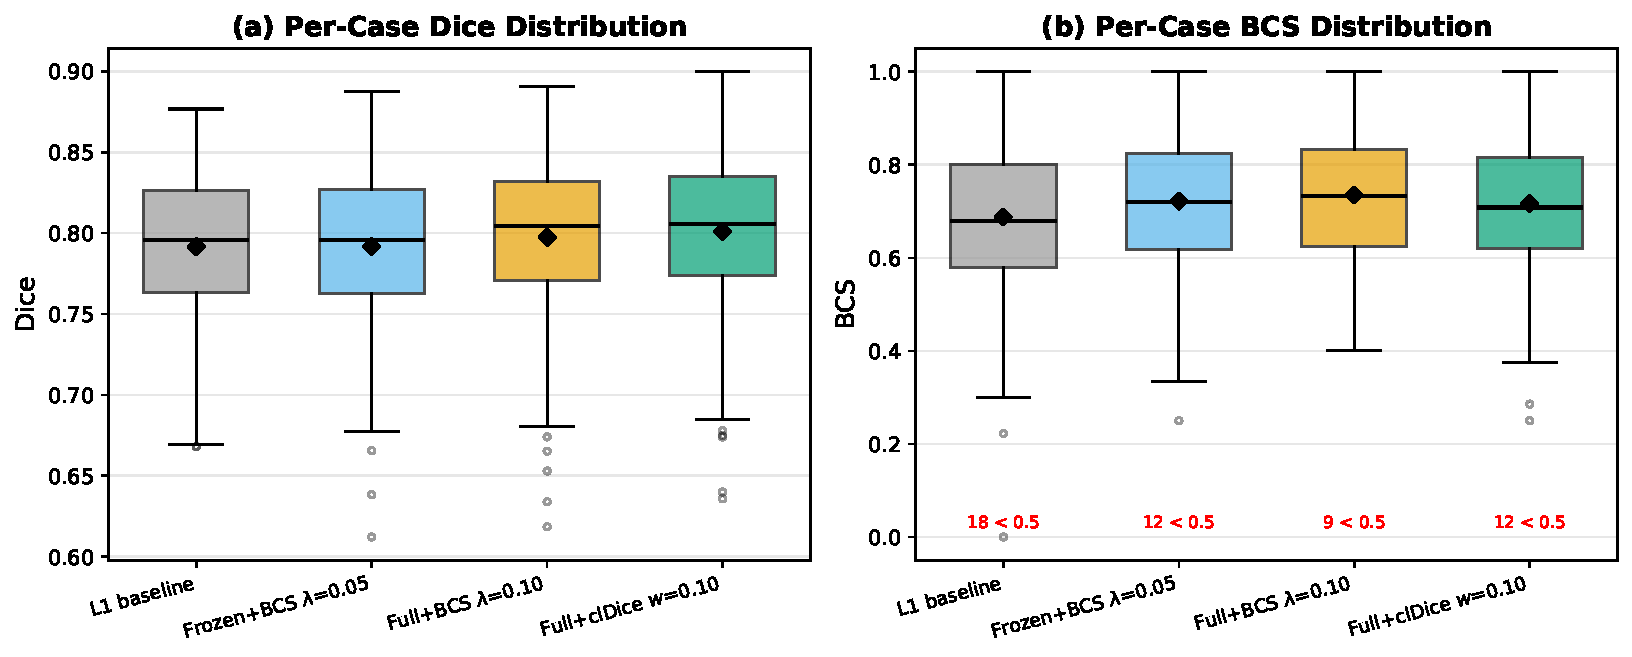
\includegraphics[width=\linewidth]{../figures/supp_per_case_distributions.pdf}
\caption{Per-case Dice and BCS distributions on ImageCAS test set ($n{=}250$). Black diamonds: mean. \textbf{(a)}~Dice distributions are similar across models, with Full+clDice showing a slight upward shift. \textbf{(b)}~Full+BCS halves the number of low-BCS outliers (BCS${<}$0.5: 9 cases vs.\ 18 for L1), confirming that BCS training targets the hardest cases.}
\label{fig:per_case}
\end{figure}

%----------------------------------------------------------------------
\section{Random-Initialisation Baseline}
\label{sec:random_init}

To quantify the contribution of domain-specific pretraining, we compare CT-FM against three randomly-initialised architectures trained on the same ImageCAS data with matched hyperparameters where feasible.

\begin{table}[h]
\caption{CT-FM vs.\ randomly-initialised architectures on ImageCAS ($n{=}250$ test). All models use freeze strategy: full fine-tuning. CT-FM achieves dramatically lower val--test gap and HD95, demonstrating that domain-specific pretraining provides an irreplaceable advantage for coronary segmentation.}
\label{tab:random_init}
\centering
\small
\begin{tabular}{llcccccc}
\toprule
Architecture & Stage & Val Dice & Test Dice & $\Delta$ & BCS & HD95\,(mm) & Betti$_0$ \\
\midrule
\textbf{CT-FM SegResNet} & L1 & 0.792 & \textbf{0.790} & 0.2\,pp & 0.690 & \textbf{8.7} & --- \\
\textbf{CT-FM SegResNet} & +BCS & 0.802 & \textbf{0.797} & 0.5\,pp & \textbf{0.735} & \textbf{6.7} & 5.7 \\
\textbf{CT-FM SegResNet} & +clDice & 0.806 & \textbf{0.801} & 0.5\,pp & 0.716 & \textbf{6.8} & 5.0 \\
\midrule
STU-Net Large & L1 & 0.825 & 0.671 & 15.4\,pp & 0.731 & 59.3 & 39.2 \\
STU-Net Large & +BCS & 0.826 & 0.689 & 13.7\,pp & 0.761 & 58.0 & 34.0 \\
\midrule
SwinUNETR & L1 & 0.812 & 0.700 & 11.2\,pp & 0.730 & 50.3 & 48.0 \\
SwinUNETR & +BCS & 0.811 & 0.716 & 9.5\,pp & 0.739 & 49.5 & 45.3 \\
\midrule
MedNeXt-B & +BCS & 0.804 & 0.673 & 13.1\,pp & 0.728 & 53.2 & 48.4 \\
\bottomrule
\end{tabular}
\end{table}

Key observations:
\begin{itemize}
\item \textbf{Val--test gap}: CT-FM exhibits a 0.2--0.5\,pp gap vs.\ 10--15\,pp for all randomly-initialised architectures, indicating severe overfitting without domain-specific pretraining.
\item \textbf{Surface precision}: CT-FM achieves HD95 $< 9$\,mm vs.\ 50--60\,mm for random-init models---a 6$\times$ improvement.
\item \textbf{BCS benefits transfer}: Two-stage BCS training improves BCS for STU-Net ($+3.0$\,pp) and SwinUNETR ($+0.9$\,pp), but cannot close the HD95 gap.
\item \textbf{Foundation model advantage}: Domain-specific CT pretraining provides an implicit ROI prior that random-init models cannot replicate with the same training data.
\end{itemize}

%----------------------------------------------------------------------
% ASOCA block (§5–§6)
%----------------------------------------------------------------------

\section{ASOCA Threshold Sweep: Full Results}
\label{sec:asoca_threshold}

Table~\ref{tab:threshold_full} presents the complete threshold sweep for all models on ASOCA ($N{=}40$). The main paper reports only the optimal threshold; here we show all evaluated thresholds.

\begin{table}[h]
\caption{ASOCA zero-shot performance across binarisation thresholds (sliding-window overlap$\,{=}\,$0.5). Dice increases monotonically with threshold while BCS remains stable (${\pm}2$\,pp), confirming that threshold calibration improves overlap at no connectivity cost. L1 outperforms Frozen+BCS at every threshold. Values at $t{=}0.5$ differ slightly from Table~5 in the main text due to different inference overlap settings.}
\label{tab:threshold_full}
\centering
\small
\begin{tabular}{llcccc}
\toprule
Model & $t$ & Dice $\uparrow$ & BCS $\uparrow$ & HD95\,(mm) $\downarrow$ & Betti$_0$ $\downarrow$ \\
\midrule
\multirow{4}{*}{L1 baseline}
 & 0.3 & 0.407 & 0.781 & 17.4 & 7.3 \\
 & 0.5 & 0.479 & 0.807 & 16.2 & 7.4 \\
 & 0.7 & 0.561 & 0.799 & 14.9 & 7.6 \\
 & 0.9 & 0.665 & 0.791 & 13.0 & 10.0 \\
\midrule
\multirow{4}{*}{Frozen $\lambda_s{=}0.05$}
 & 0.3 & 0.370 & 0.815 & 24.5 & 16.9 \\
 & 0.5 & 0.444 & 0.822 & 21.5 & 14.1 \\
 & 0.7 & 0.532 & 0.812 & 18.5 & 12.7 \\
 & 0.9 & 0.655 & 0.815 & 14.7 & 12.6 \\
\bottomrule
\end{tabular}
\end{table}

%----------------------------------------------------------------------
\section{ASOCA Normal vs.\ Diseased Breakdown}
\label{sec:asoca_subgroups}

\begin{table}[h]
\caption{ASOCA subgroup analysis: Normal ($n{=}20$) vs.\ Diseased ($n{=}20$) at $t{=}0.5$ for zero-shot models, and $n{=}17$ per group for $k{=}1$ (3 per group used for training). Diseased cases show lower BCS due to calcified plaque disrupting connectivity, while normal cases show lower Dice due to more extensive side-branch over-segmentation.}
\label{tab:asoca_subgroups}
\centering
\small
\begin{tabular}{llcccc}
\toprule
Model & Subgroup & Dice $\uparrow$ & BCS $\uparrow$ & HD95\,(mm) $\downarrow$ \\
\midrule
\multirow{2}{*}{L1 baseline}
 & Normal   & 0.456 & 0.877 & 14.7 \\
 & Diseased & 0.505 & 0.710 & 16.8 \\
\midrule
\multirow{2}{*}{Frozen $\lambda_s{=}0.05$}
 & Normal   & 0.432 & 0.852 & 18.8 \\
 & Diseased & 0.459 & 0.796 & 23.3 \\
\midrule
\multirow{2}{*}{$k{=}1$ best ($n_{\mathrm{eval}}{=}34$)}
 & Normal   & 0.771 & 0.798 & 28.9 \\
 & Diseased & 0.653 & 0.615 & 41.1 \\
\bottomrule
\end{tabular}
\end{table}

\end{document}
